\documentclass{article}
\usepackage[utf8]{inputenc}
\usepackage{fancyhdr}
\usepackage{lastpage}
\usepackage{amsfonts}
\usepackage{amsmath}
\usepackage{amsthm}
\usepackage{amssymb}
\usepackage{bm}
\usepackage{csquotes}
\usepackage{mymacros}
\usepackage{graphicx}
\usepackage{geometry}
\usepackage{mathtools}
\usepackage[shortlabels]{enumitem}
\usepackage[noabbrev, capitalise]{cleveref}

\usepackage{geometry}
 \geometry{
 a4paper,
 top=20mm,
 bottom=25mm,
 left=25mm,
 right=25mm,
 }

% define your IDs here:
\newcommand{\firststudentid}{205679863}
\newcommand{\secondstudentid}{311151138}
\newcommand{\thirdstudentid}{318635646}

\pagestyle{fancy}
\fancyhf{}
\rhead{Solution for Assignment 2}
\chead{\firststudentid \qquad \secondstudentid \qquad \thirdstudentid}
\lhead{Natural Language Processing}
\rfoot{Page \thepage \hspace{1pt} of \pageref{LastPage}}
\renewcommand{\footrulewidth}{1pt}
 
\setlength{\parindent}{0pt}
\setlength{\parskip}{1em}
\renewcommand{\baselinestretch}{1.25}

\renewcommand{\thesubsection}{\thesection.\alph{subsection}}
\renewcommand{\thesubsubsection}{\thesubsection.\roman{subsubsection}}

\begin{document}

\section{Word-Level Neural Bi-gram Language Model}
\subsection{}
\begin{proof}
  Let $\bm{x} \in \R^d$ be an input vector and let $c \in \R$ be some constant. For any $i \in [d]$ it holds that:  
  \begin{equation*}
    \begin{split}
      (\text{softmax}(\bm{x} + c))_i & = \frac{\exp(x_i + c)}{\sum_{j = 1}^{d} \exp(x_j + c)} \\
      & = \frac{e^c \exp(x_i)}{e^c \sum_{j = 1}^{d} \exp(x_j)} \\
      & = \frac{\exp(x_i)}{\sum_{j = 1}^{d} \exp(x_j)} \\
      & = (\text{softmax}(\bm{x}))_i
    \end{split}
  \end{equation*}
\end{proof}

\subsection{}
\begin{proof}
  Note that the true empirical distribution $\bm{y}$ is a one-hot vector with a 1 for the true outside word o, and 0 everywhere else, thus:
  \begin{equation*}
    -\sum\limits_{w \in \text{W}} y_w \log(\hat{y}_w) = -\sum\limits_{w \in \text{W}} \I{o}(w) \log(\hat{y}_w) = \log(\hat{y}_o)
  \end{equation*}
\end{proof}

\setcounter{subsection}{3}
\subsection{}
\begin{enumerate}
  [label=(\roman*)]
  \item ${\frac{\partial \bm J_{\textrm{skip-gram}}(c, w_{t-m},\ldots w_{t+m}, \bm V, \bm U)} {\partial \bm U}} = \sum_{\substack{-m \le j \le m \\ j \ne 0}} \frac{\partial \bm{J} (\bm{v_c},w_{t+j},\bm{U})}{\partial \bm{U}}  $
  \item ${\frac{\partial \bm J_{\textrm{skip-gram}}(c, w_{t-m},\ldots w_{t+m}, \bm V, \bm U)} {\partial \bm v_c}} = \sum_{\substack{-m \le j \le m \\ j \ne 0}} \frac{\partial \bm{J} (\bm{v_c},w_{t+j},\bm{U})}{\partial \bm{v_c}}  $
  \item Assuming $\bm J_{\textrm{skip-gram}}(c, w_{t-m},\ldots w_{t+m}, \bm V, \bm U)$ is not a function of $\bm v_c$ when $w \ne c$: \\
   ${\frac{\partial \bm J_{\textrm{skip-gram}}(c, w_{t-m},\ldots w_{t+m}, \bm V, \bm U)} {\partial \bm v_w}} = \bm 0$ 
\end{enumerate}


\section{Theoretical Inquiry of a Simple RNN Language Model}
\subsection{}
The notation used in the question is incorrect, we assume all vectors are "column" vectors e.g. $h^{(t)} \in \R^{D_h}$, and that the appropriate transposed were omitted in the question.  

\subsubsection[short]{$\frac{\partial J^{(t)}}{\partial U}(\theta)$}
First we compute $\frac{\partial J^{(t)}}{\partial U}(\theta)$. 
Recall that because $y^{(t)}$ is a one-hot vector our loss simplifies to:
\begin{equation}
  J^{(t)}(\theta) = -{y_k}^{(t)} \log {\hat{y}_k}^{(t)}
\end{equation}
where $k$ is the index of the target word in the vocabulary.\\

Next, let us denote ${o^{(t)}}^T = {h^{(t)}}^T U + b_2^T$, recall our previous computation of the differential of the cross entropy loss with a one-hot vector:
\begin{equation} \label{eq:grad_o}
  \frac{\partial J^{(t)}}{\partial o^{(t)}}(\theta) = \hat{y}^{(t)} - y^{(t)}
\end{equation}
Furthermore we have:
\begin{equation}
  \frac{\partial o_l^{(t)}}{\partial U_{i,j}}(\theta) = \I{l=j} h^{(t)}_i
\end{equation}
Combining the last results yields:
\begin{equation}
  \frac{\partial J^{(t)}}{\partial U_{i,j}}(\theta) =  h^{(t)}_i (\hat{y}^{(t)} - y^{(t)})_j
\end{equation}
which is recognizable as the outer product:
\begin{equation}
  \boxed{ \frac{\partial J^{(t)}}{\partial U}(\theta) =  h^{(t)} \otimes (\hat{y}^{(t)} - y^{(t)}) } 
\end{equation}

\subsubsection[short]{$\frac{\partial J^{(t)}}{\partial L_{x^{(t)}}}(\theta)$}
Next we compute $\frac{\partial J^{(t)}}{\partial L_{x^{(t)}}}(\theta)$, note that this gradient must be back-propagated through time, but we defer it to section b. 
Again applying the chain rule we have:
\begin{equation} \label{eq:grad_L}
  \frac{\partial J^{(t)}}{\partial L_{i,j}}(\theta) = \frac{\partial J^{(t)}}{\partial \hat{y}^{(t)}} \frac{{\partial \hat{y}^{(t)}}}{\partial o^{(t)}} \frac{\partial o^{(t)}}{\partial h^{(t)}} \frac{\partial h^{(t)}}{\partial L_{i,j}} 
\end{equation}

where $\frac{\partial J^{(t)}}{\partial \hat{y}^{(t)}} \frac{{\partial \hat{y}^{(t)}}}{\partial o^{(t)}} = \frac{\partial J^{(t)}}{\partial o^{(t)}} = \hat{y}^{(t)} - y^{(t)}$ was already computed in (\ref{eq:grad_o}). 
The third term in (\ref{eq:grad_L}) is immediate by the definition of the differential of a linear function:
\begin{equation} \label{eq:grad_o_by_h}
  \frac{\partial o_l^{(t)}}{\partial h_m^{(t)}} = (U^T)_{l,m} = U_{m,l}
\end{equation}

Lastly we derive the fourth term in (\ref{eq:grad_L}) using the chain-rule without unfolding through time.
Let us denote $a^{(t)} = H^T h^{(t-1)} +I^T e^{(t)} + b_1^T$, then:
\begin{equation} \label{eq:grad_h_by_L}
  \begin{aligned}
    \frac{\partial h^{(t)}}{\partial L_{i,j}} &= \frac{\partial \sigma}{\partial a^{(t)}} \left( \frac{\partial}{\partial L_{i,j}} { \left(L_{x^{(t)}}I \right)}  + \frac{\partial }{\partial L_{i,j}} \left( {h^{(t-1)}}^T H \right) \right) \\
  \end{aligned}
\end{equation}

For this section, we make the simplifying assumption that $x^{(t_1)} \neq x^{(t_2)}$ for any $t_1 \neq t_2$, as implied in the question,
which implies that $ \frac{\partial }{\partial L_{x^{(t)}}} \left( {h^{(t-1)}}^T H \right) = 0$ .

Recalling the derivative of the sigmoid yields:
\begin{equation}
  \frac{\partial \sigma_k(a^{(t)})}{\partial a^{(t)}_l}(\theta) = \sigma (a^{(t)}_k) \left(1 - a^{(t)}_k \right) \frac{\partial a^{(t)}_k}{\partial a^{(t)}_l}
\end{equation}

Thus we have:
\begin{equation}
  \frac{\partial \sigma(a^{(t)})}{\partial a^{(t)}}(\theta) = \text{diag}\left[ h^{(t)} \right]  \text{diag}\left[ \vec{1} - h^{(t)} \right] 
\end{equation}

A simple computation yields:
\begin{equation}
  \frac{\partial}{\partial L_{x^{(t)}}} { \left(L_{x^{(t)}}I \right)} = I^T
\end{equation}

Plugging the above computations into (\ref{eq:grad_L}) gives:
\begin{equation} \label{eq:grad_L_final}
  \boxed{ \frac{\partial J^{(t)}}{\partial L_{x^{(t)}}}(\theta) = \left(\hat{y}^{(t)} - y^{(t)}\right)^T U^T \; \text{diag}\left[ h^{(t)} \right] \text{diag}\left[ \vec{1} - h^{(t)} \right] I^T }
\end{equation}


\subsubsection[short]{$ \frac{\partial J^{(t)}}{\partial I}(\theta) $}

In a similar fashion to (\ref{eq:grad_L}), we apply the chain rule:
\begin{equation} \label{eq:grad_I_chainrule}
  \frac{\partial J^{(t)}}{\partial I_{i,j}}(\theta) = \frac{\partial J^{(t)}}{\partial \hat{y}_k^{(t)}} \frac{{\partial \hat{y}_k^{(t)}}}{\partial o_l^{(t)}} \frac{\partial o_l^{(t)}}{\partial h^{(t)}} \frac{\partial h^{(t)}}{\partial I_{i,j}} 
\end{equation}

Note that only the last term in (\ref{eq:grad_I}) differs from (\ref{eq:grad_L}), futhermore in a similar fashion to (\ref{eq:grad_h_by_L}):
\begin{equation} \label{eq:grad_h_by_I}
  \frac{\partial h^{(t)}}{\partial I_{i,j}} = \frac{\partial \sigma}{\partial a^{(t)}} \left( \frac{\partial}{\partial I_{i,j}} { \left({e^{(t)}}^T I \right)}  + \frac{\partial }{\partial I_{i,j}} \left( {h^{(t-1)}}^T H \right) \right) \\
\end{equation}

Again a simple computation yields:
\begin{equation}
  \frac{\partial}{\partial I_{i,j}} { \left({e^{(t)}}^T I \right)} = e^{(t)}_i \cdot \textbf{\text{e}}_j
\end{equation}

Plugging this into (\ref{eq:grad_I_chainrule}), assuming $h^{(t-1)}$ is constant in $I$:
\begin{equation} \label{eq:grad_I_ij}
  \restr{\frac{\partial J^{(t)}}{\partial I_{i,j}}}{(t)}(\theta) = \left(\hat{y}^{(t)} - y^{(t)}\right)^T U^T \; \text{diag}\left[ h^{(t)} \right]  \text{diag}\left[ \vec{1} - h^{(t)} \right] e^{(t)}_i \cdot \textbf{\text{e}}_j
\end{equation}

Recognizing the above form as the outer product:
\begin{equation} \label{eq:grad_I}
  \boxed{ \restr{\frac{\partial J^{(t)}}{\partial I}}{(t)}(\theta) = e^{(t)} \otimes \left(\left(\hat{y}^{(t)} - y^{(t)}\right)^T U^T \; \text{diag}\left[ h^{(t)} \right]  \text{diag}\left[ \vec{1} - h^{(t)} \right] \right)^T }
\end{equation}


\subsubsection[short]{$ \frac{\partial J^{(t)}}{\partial H}(\theta) $}
In a similar fashion to (\ref{eq:grad_L}), we apply the chain rule:
\begin{equation} \label{eq:grad_H_chainrule}
  \frac{\partial J^{(t)}}{\partial H_{i,j}}(\theta) = \frac{\partial J^{(t)}}{\partial \hat{y}_k^{(t)}} \frac{{\partial \hat{y}_k^{(t)}}}{\partial o_l^{(t)}} \frac{\partial o_l^{(t)}}{\partial h^{(t)}} \frac{\partial h^{(t)}}{\partial H_{i,j}} 
\end{equation}

Note that only the last term in (\ref{eq:grad_I}) differs from (\ref{eq:grad_L}), futhermore in a similar fashion to (\ref{eq:grad_h_by_L}):
\begin{equation} \label{eq:grad_h_by_H}
  \frac{\partial h^{(t)}}{\partial H_{i,j}} = \frac{\partial \sigma}{\partial a^{(t)}} \left(  \frac{\partial }{\partial H_{i,j}} \left( {h^{(t-1)}}^T H \right) \right) \\
\end{equation}
where 
\begin{equation}
  \frac{\partial }{\partial H_{i,j}} \left( {h^{(t-1)}}^T H \right) = H^T \left( \frac{\partial h^{(t-1)}}{\partial H_{i,j}} \right) \;+\; h^{(t-1)}_i \cdot \textbf{\text{e}}_j
\end{equation}

Focusing on the t-th appearence of $H$:
\begin{equation}
  \restr{\frac{\partial }{\partial H_{i,j}}}{(t)}\left( {h^{(t-1)}}^T H \right) = h^{(t-1)}_i \cdot \textbf{\text{e}}_j
\end{equation}

And in a similar fashion to (\ref{eq:grad_I})
\begin{equation} \label{eq:grad_H}
  \boxed{ \restr{\frac{\partial J^{(t)}}{\partial H}}{(t)}(\theta) = h^{(t-1)} \otimes \left(\left(\hat{y}^{(t)} - y^{(t)}\right)^T U^T \; \text{diag}\left[ h^{(t)} \right]  \text{diag}\left[ \vec{1} - h^{(t)} \right] \right)^T }
\end{equation}



\subsubsection[short]{$ \frac{\partial J^{(t)}}{\partial h^{(t-1)}}(\theta) $}

In a similar fashion to (\ref{eq:grad_L}), we apply the chain rule:
\begin{equation} \label{eq:grad_h_prev_chainrule}
  \frac{\partial J^{(t)}}{\partial h^{(t-1)}}(\theta) = \frac{\partial J^{(t)}}{\partial \hat{y}_k^{(t)}} \frac{{\partial \hat{y}_k^{(t)}}}{\partial o_l^{(t)}} \frac{\partial o_l^{(t)}}{\partial h^{(t)}} \frac{\partial h^{(t)}}{\partial h^{(t-1)}} 
\end{equation}

where again only $\frac{\partial h^{(t)}}{\partial h^{(t-1)}}$ is yet to be computed, and is given by:
\begin{equation} 
  \frac{\partial h^{(t)}}{\partial h^{(t-1)}} = H^T
\end{equation}

Plugging this into (\ref{eq:grad_h_prev_chainrule}) yields:
\begin{equation} \label{eq:grad_h_prev}
  \boxed{ \frac{\partial J^{(t)}}{\partial h^{(t-1)}}(\theta) = \left(\hat{y}^{(t)} - y^{(t)}\right)^T U^T \; \text{diag}\left[ h^{(t)} \right]  \text{diag}\left[ \vec{1} - h^{(t)} \right] H^T }
\end{equation}


\subsection{}
\begin{figure}
  \centering
  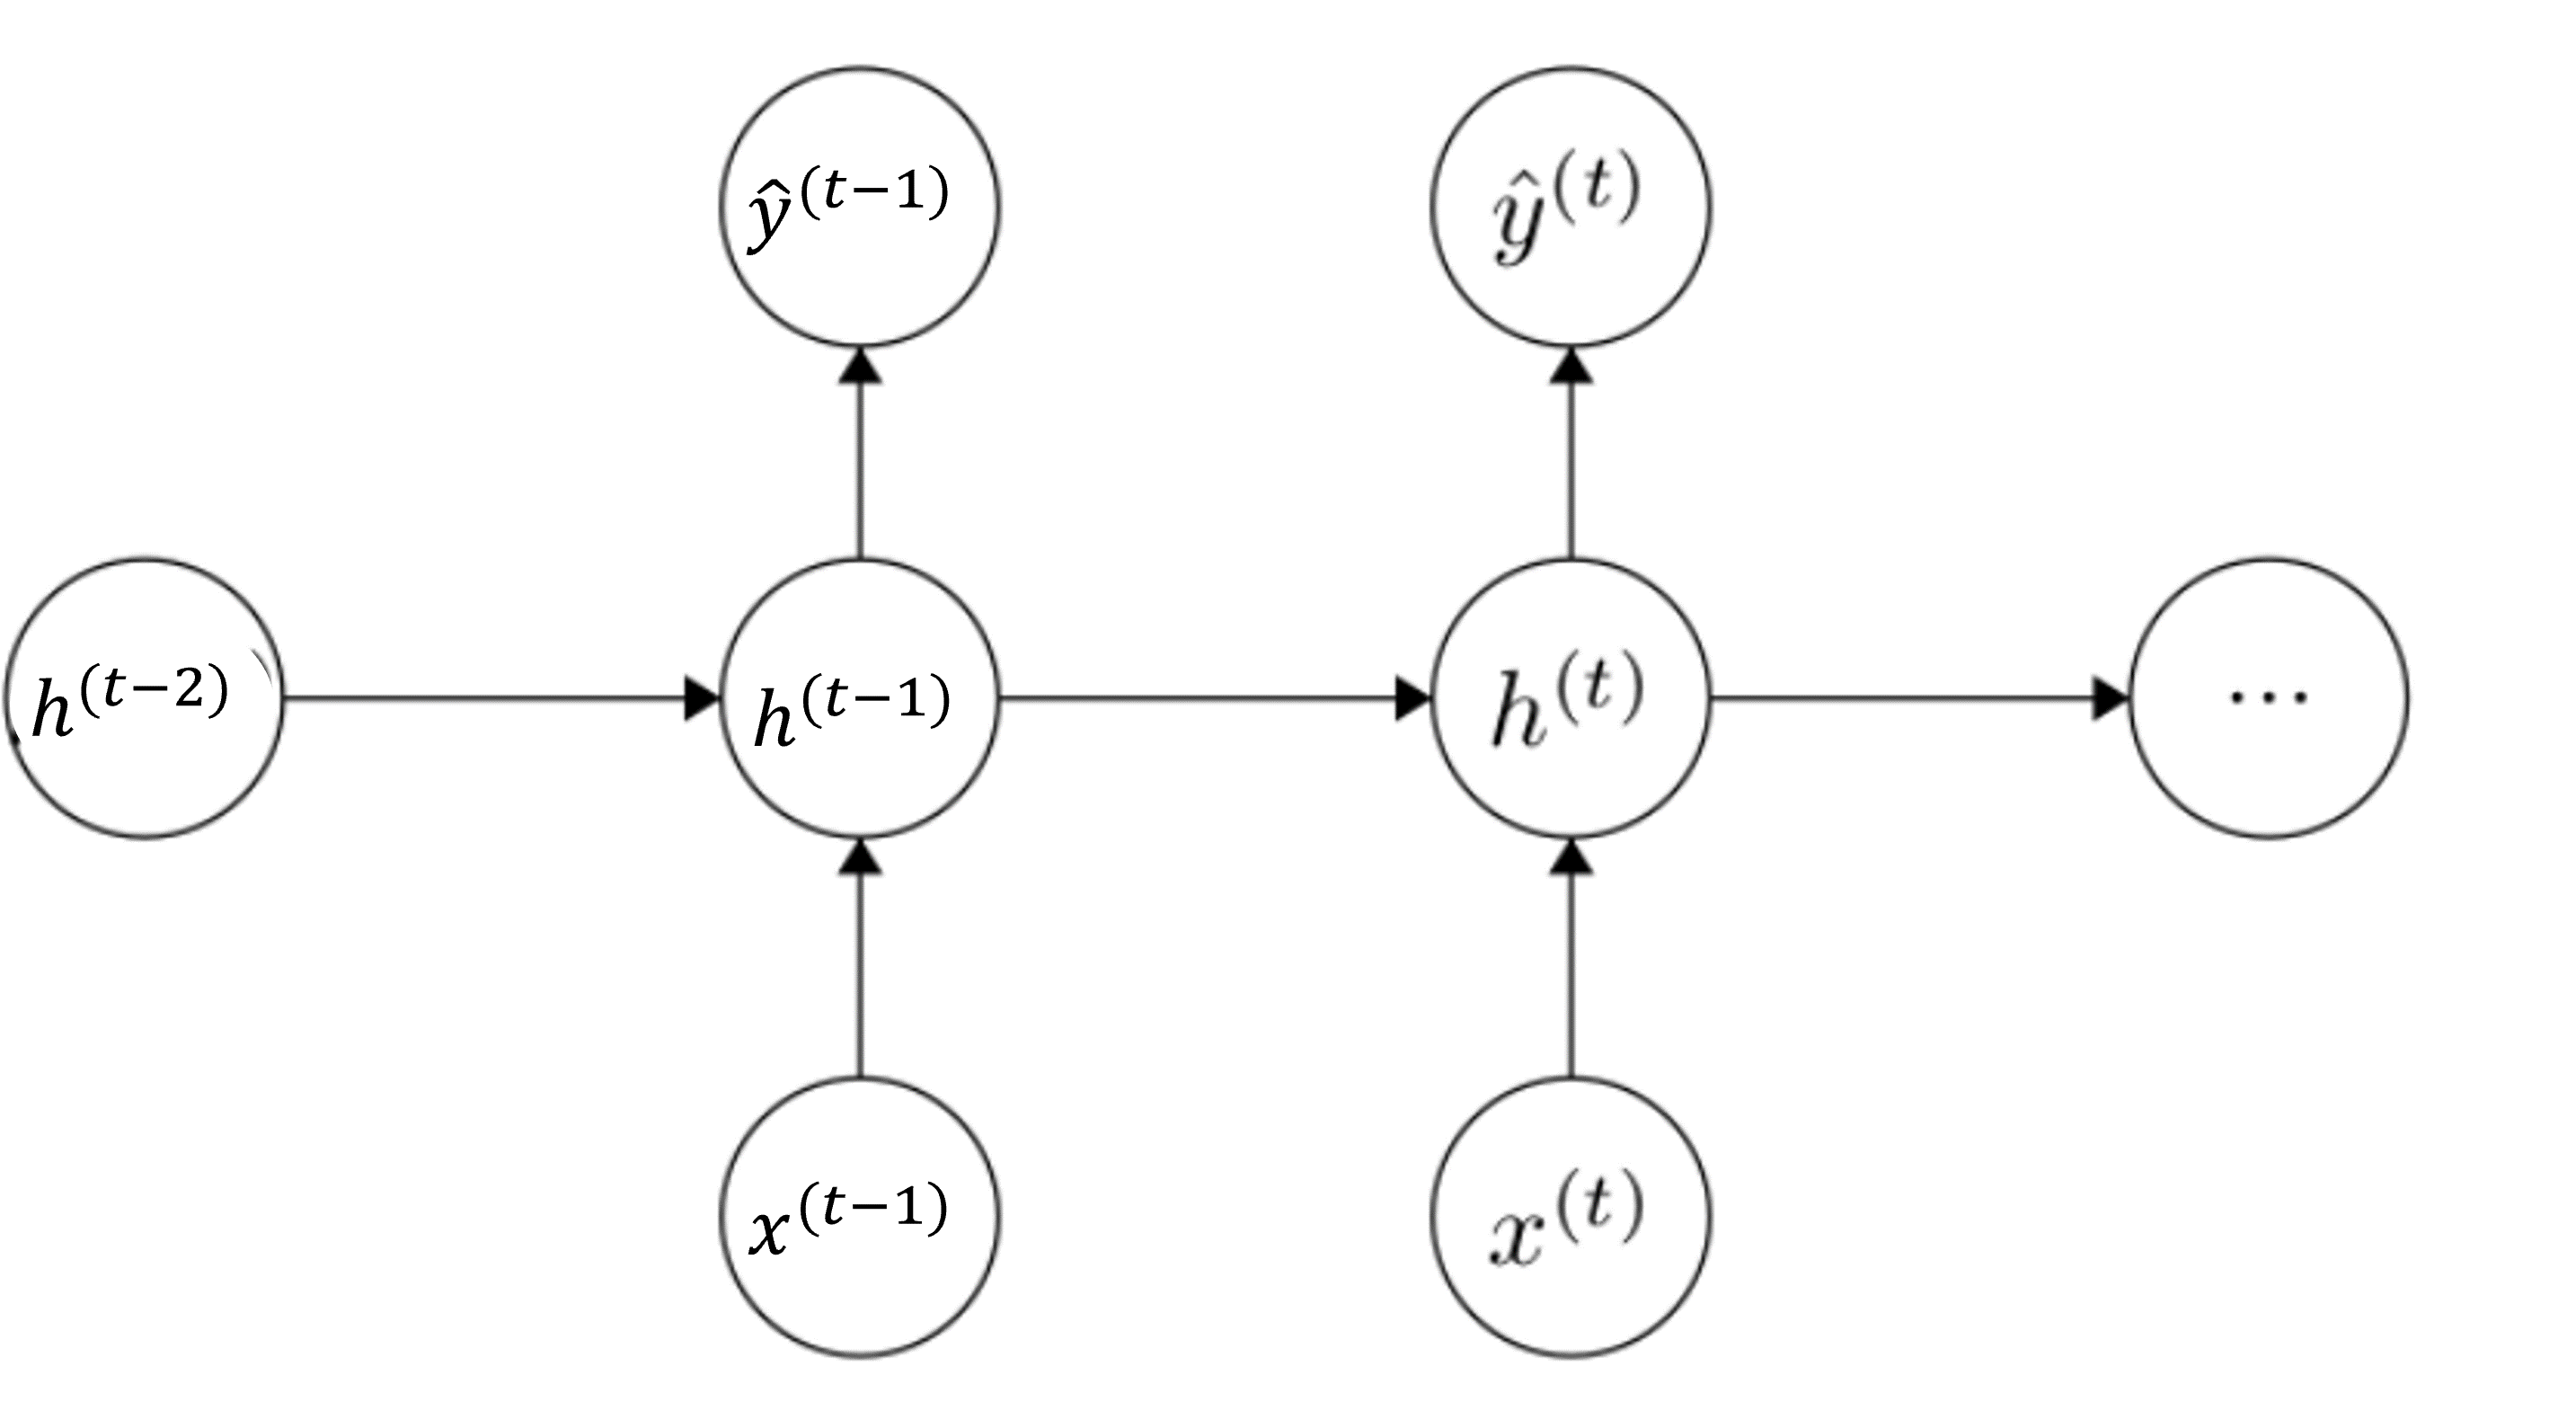
\includegraphics[width=0.9\linewidth]{q2/RNN_graph_updated.png}
  \label{fig:RNN_graph}
\end{figure}

We now backpropagate 1 step through time, expressing out answer using the terms requested in part (a).

\subsubsection[short]{$\frac{\partial J^{(t)}}{\partial L_{x^{(t-1)}}}(\theta)$}
Looking at equation (\ref{eq:grad_h_by_L}) shows us that:

\begin{equation} \label{eq:grad_h_by_L_induction_step}
  \begin{aligned}
    \frac{\partial h^{(t)}}{\partial L_{i,j}} &= \frac{\partial \sigma}{\partial a^{(t)}} \left( \frac{\partial}{\partial L_{i,j}} { \left(L_{x^{(t)}}I \right)}  + \frac{\partial }{\partial L_{i,j}} \left( {h^{(t-1)}}^T H \right) \right) \\
    &= \restr{\frac{\partial h^{(t)}}{\partial L_{i,j}}}{(t)} + \; \frac{\partial h^{(t)}}{\partial h^{(t-1)}} \cdot \frac{\partial h^{(t-1)}}{\partial L_{i,j}}
  \end{aligned}
\end{equation}

We can unroll one timestamp further into the past $(t-2)$ by applying the chain rule once again:
\begin{equation}
  \frac{\partial h^{(t-1)}}{\partial L_{i,j}} = \restr{\frac{\partial h^{(t-1)}}{\partial L_{i,j}}}{(t-1)} +\; \frac{\partial h^{(t-1)}}{\partial h^{(t-2)}} \cdot \frac{\partial h^{(t-2)}}{\partial L_{i,j}}
\end{equation}

Plugging this expression back into (\ref{eq:grad_h_by_L_induction_step}) gives:
\begin{equation}
  \begin{aligned}
    \frac{\partial h^{(t)}}{\partial L_{i,j}} &= \restr{\frac{\partial h^{(t)}}{\partial L_{i,j}}}{(t)} +\; \frac{\partial h^{(t)}}{\partial h^{(t-1)}} \left( \restr{\frac{\partial h^{(t-1)}}{\partial L_{i,j}}}{(t-1)} +\; \frac{\partial h^{(t-1)}}{\partial h^{(t-2)}} \cdot \frac{\partial h^{(t-2)}}{\partial L_{i,j}} \right) \\
    &= \restr{\frac{\partial h^{(t)}}{\partial L_{i,j}}}{(t)} +\; \frac{\partial h^{(t)}}{\partial h^{(t-1)}} \cdot \restr{\frac{\partial h^{(t-1)}}{\partial L_{i,j}}}{(t-1)} +\; \frac{\partial h^{(t)}}{\partial h^{(t-2)}} \cdot \frac{\partial h^{(t-2)}}{\partial L_{i,j}} \\
    &= \sum_{l=t-1}^{t}  \frac{\partial h^{(t)}}{\partial h^{(l)}} \cdot \restr{\frac{\partial h^{(l)}}{\partial L_{i,j}}}{(l)} \; + \; \frac{\partial h^{(t)}}{\partial h^{(t-2)}} \cdot \frac{\partial h^{(t-2)}}{\partial L_{i,j}}
  \end{aligned}
\end{equation}

Which using our notation yields:
\begin{equation}
  \begin{aligned}
    \frac{\partial J^{(t)}}{\partial L_{i,j}}(\theta) &= \sum_{l=t-1}^{t} \frac{\partial J^{(t)}}{\partial h^{(l)}} \cdot \restr{\frac{\partial h^{(l)}}{\partial L_{i,j}}}{(l)} \;+\; \frac{\partial J^{(t)}}{\partial h^{(t-2)}} \cdot \frac{\partial h^{(t-2)}}{\partial L_{i,j}} \\
    &= \sum_{l=t-1}^{t} \frac{\partial J^{(t)}}{\partial h^{(l)}} \cdot \restr{\frac{\partial h^{(l)}}{\partial L_{i,j}}}{(l)} \;+\; \frac{\partial J^{(t-2)}}{\partial L_{i,j}}
  \end{aligned}
\end{equation}

Substituting in for $\partial L_{x^{(t-1)}}$:
\begin{equation}
  \frac{\partial J^{(t)}}{\partial L_{x^{(t-1)}}}(\theta) = \sum_{l=t-1}^{t} \frac{\partial J^{(t)}}{\partial h^{(l)}} \cdot \restr{\frac{\partial h^{(l)}}{\partial L_{x^{(t-1)}}}}{(l)} \;+\; \frac{\partial J^{(t-2)}}{\partial L_{x^{(t-1)}}}
\end{equation}

where $\restr{\frac{\partial h^{(l)}}{\partial L_{x^{(t-1)}}}}{(l)} = 0$ whenever $x^{(l)} \neq x^{(t-1)}$. For simplicity, again assuming $x^{(t_1)} \neq x^{(t_2)}$ for any $t_1 \neq t_2$ gives:
\begin{equation}
    \boxed{ \frac{\partial J^{(t)}}{\partial L_{x^{(t-1)}}}(\theta) = \frac{\partial J^{(t)}}{\partial h^{(t-1)}} \cdot \restr{\frac{\partial h^{(t-1)}}{\partial L_{x^{(t-1)}}}}{(t-1)} }
\end{equation}

Or explicitly:
\begin{equation}
  \frac{\partial J^{(t)}}{\partial L_{x^{(t-1)}}}(\theta) = \left(\hat{y}^{(t)} - y^{(t)}\right)^T U^T \; \text{diag}\left[ h^{(t)} \right]  \text{diag}\left[ \vec{1} - h^{(t)} \right] H^T \text{diag}\left[ h^{(t-1)} \right]  \text{diag}\left[ \vec{1} - h^{(t-1)} \right] I^T 
\end{equation}


\subsubsection[short]{$\restr{\frac{\partial J^{(t)}}{\partial H}}{(t-1)}$}

By applying the same derivations such as in (\ref{eq:grad_h_by_H}):
\begin{equation}
  \begin{aligned}
    \restr{\frac{\partial J^{(t)}}{\partial H_{i,j}}}{(t-1)} &= \frac{\partial J^{(t)}}{\partial h^{(t-1)}} \cdot \restr{\frac{\partial h^{(t-1)}}{\partial H_{i,j}}}{(t-1)} \\
    &= \frac{\partial J^{(t)}}{\partial h^{(t-1)}} \cdot \text{diag}\left[ h^{(t-1)} \right]  \text{diag}\left[ \vec{1} - h^{(t-1)} \right] h^{(t-2)}_i \cdot \textbf{\text{e}}_j
  \end{aligned}
\end{equation}

which is reconized as the outer product:
\begin{equation}
  \boxed {\restr{\frac{\partial J^{(t)}}{\partial H}}{(t-1)} = h^{(t-2)} \otimes \left( \frac{\partial J^{(t)}}{\partial h^{(t-1)}} \cdot \text{diag}\left[ h^{(t-1)} \right]  \text{diag}\left[ \vec{1} - h^{(t-1)} \right] \right)^T }
\end{equation}

Or explicitly:
\begin{equation}
  \restr{\frac{\partial J^{(t)}}{\partial H}}{(t-1)} = h^{(t-2)} \otimes \left( \left(\hat{y}^{(t)} - y^{(t)}\right)^T U^T \; \text{diag}\left[ h^{(t)} \right]  \text{diag}\left[ \vec{1} - h^{(t)} \right] H^T \text{diag}\left[ h^{(t-1)} \right]  \text{diag}\left[ \vec{1} - h^{(t-1)} \right] \right)^T
\end{equation}


\subsubsection[short]{$\restr{\frac{\partial J^{(t)}}{\partial I}}{(t-1)}$}
In a similar fashion to the previous derivation:
\begin{equation}
  \boxed {\restr{\frac{\partial J^{(t)}}{\partial I}}{(t-1)} = e^{(t-1)} \otimes \left( \frac{\partial J^{(t)}}{\partial h^{(t-1)}} \cdot \text{diag}\left[ h^{(t-1)} \right]  \text{diag}\left[ \vec{1} - h^{(t-1)} \right] \right)^T }
\end{equation}


\subsubsection[short]{$\restr{\frac{\partial J^{(t)}}{\partial b_1}}{(t-1)}$}

\begin{equation}
  \begin{aligned}
    \restr{\frac{\partial J^{(t)}}{\partial b_1}}{(t-1)} &= \frac{\partial J^{(t)}}{\partial h^{(t-1)}} \cdot \restr{\frac{\partial h^{(t-1)}}{\partial b_1}}{(t-1)} \\
    &= \Aboxed{ \frac{\partial J^{(t)}}{\partial h^{(t-1)}} \cdot \text{diag}\left[ h^{(t-1)} \right]  \text{diag}\left[ \vec{1} - h^{(t-1)} \right] } 
  \end{aligned}
\end{equation}

\section{Generating Shakespeare Using a Character-level Language Model}
\subsection{}
\begin{proof}
    Using the first hint, we can rewrite our objection as follows:
    \begin{equation*}
            \mathcal{L}(\theta) = \prod_{c,o} p_{\theta}(o|c)^{\#(c,o)}
    \end{equation*}
    This is true because the term $p_\theta(o|c)$ by definition will appear $\#(c,o)$ times.
    Notice that for a center word $c$, the distribution of $p_theta(o|c)$ is independent from $p_\theta(o|\hat{c})$ where $c\neq\hat{c}$.
    So, we can split $\cal{L}(\theta)$ into $\cal{L}$$_c(\theta)$ such that:
    \begin{equation*}
            \mathcal{L}_c(\theta) = \prod_{o} p_{\theta}(o|c)^{\#(c,o)}
    \end{equation*}
    Taking a logarithm we get:
    \begin{equation*}
            J_c(\theta) = \sum_{o} \#(c,o)\log{p_{\theta}(o|c)}
    \end{equation*}

    Since for each $c$, $p_theta(o|c)$ is a probability distribution, we know that:
    \begin{equation*}
            \sum_{o}p_{\theta}(o|c)=1
    \end{equation*}
    So we want to solve: $J_c(\theta) = \sum_{o} \#(c,o)\log{p_{\theta}(o|c)}$ s.t $\sum_{o}p_{\theta}(o|c)=1$  and  $p_{\theta}(o|c)\ge0$

    We will solve it using Lagrange multipliers:
    \begin{equation*}
        \begin{split}
            L_c(\theta,\lambda)=\sum_{o}\#(c,o)\log{p_{\theta}(o|c)}-\lambda(\sum_{o}p_{\theta}(o|c)-1)
        \end{split}
    \end{equation*}
    \begin{equation*}
        \begin{split}
            \frac{\partial L_c}{\partial p_{\theta}(o|c)}=\frac{\#(c,o)}{p_{\theta}(o|c)}-\lambda
        \end{split}
    \end{equation*}

    So: 
    \begin{equation*}
        \frac{\partial L_c}{\partial p_{\theta}(o|c)}=0\rightarrow p_{\theta}(o|c)=\frac{\#(c,o)}{\lambda}
    \end{equation*}

    Now we can find $\lambda$ using the constrains:
    
    \begin{equation*}
        \sum_{o} p_\theta(o|c)= \sum_{o}\frac{\#(c,o)}{\lambda}=1
    \end{equation*}
    Which means that:
    \begin{equation*}
        \lambda = \sum_{o}\#(c,o)
    \end{equation*}
    So finally:
    \begin{equation*}
        p_\theta(o|c) = \frac{\#(c,o)}{\sum_{o'}\#(c,o')}
    \end{equation*}
    as desired.
\end{proof}


\section{Perplexity}
\subsection{}
\begin{align*}
    &2^{-\frac{1}{M}\sum log_2 p(s_i | s_1,...,s_{i-1})}= \\
&= (2^{\sum log_2 p(s_i | s_1,...,s_{i-1})})^{-\frac{1}{M}}= \\
&= (\prod 2^{log_2 p(s_i | s_1,...,s_{i-1})})^{-\frac{1}{M}}= \\
&= (\prod p(s_i | s_1,...,s_{i-1}))^{-\frac{1}{M}}= \\
&= (\prod e^{ln p(s_i | s_1,...,s_{i-1})})^{-\frac{1}{M}}= \\
&= e^{-\frac{1}{M}\sum ln p(s_i | s_1,...,s_{i-1})}
\end{align*}
\subsection{}
The simplest solution is to remove the relus, i.e $\sigma(x_1^T x_2)$.
If we have to keep the relu functions at the last layer, then we can map the sigmoid into $[0,1]$ by adding this computation
$$2*(\sigma (relu(x_1)^T relu(x_2)) - 0.5)$$
\subsection{}
There are two insights that we conclude from the results. First, the RNN seems to be better at predicting the next word than the Bi-Gram model for both of the datasets, as we can see from its lower perplexity values.
Second, the perplexity of the RNN is lower for the Shakespeare dataset than for the Wikipedia dataset, this is true for the Bi-Gram model as well.

The first insight can be explained by the fact the RNN is not a bigram model, i.e each character prediction depends (theoretically, at least) on all the previous characters, while the Bi-Gram model only depends on the previous character. 
We've seen in class (and understand intuitively) that the markovian assumption that underlies the bigram model does not hold in reality.

The second insight can be explained by the fact that the RNN was trained on Shakespeare text, hence we can expcet it to be better in a similar task, i.e another Shakespeare text. That's probably not the whole story, as we can see that the 
bigram model, which wasn't trained on Shakespeare text, has lower perplexity on the Shakespeare text as well. This may be because the Wikipedia text may be "harder" in a sense, for example it may contain more facts and less
stylistic text, which may be harder to predict (even for LLM facts are problematic).



\section{Deep Averaging Networks}
\subsection{}
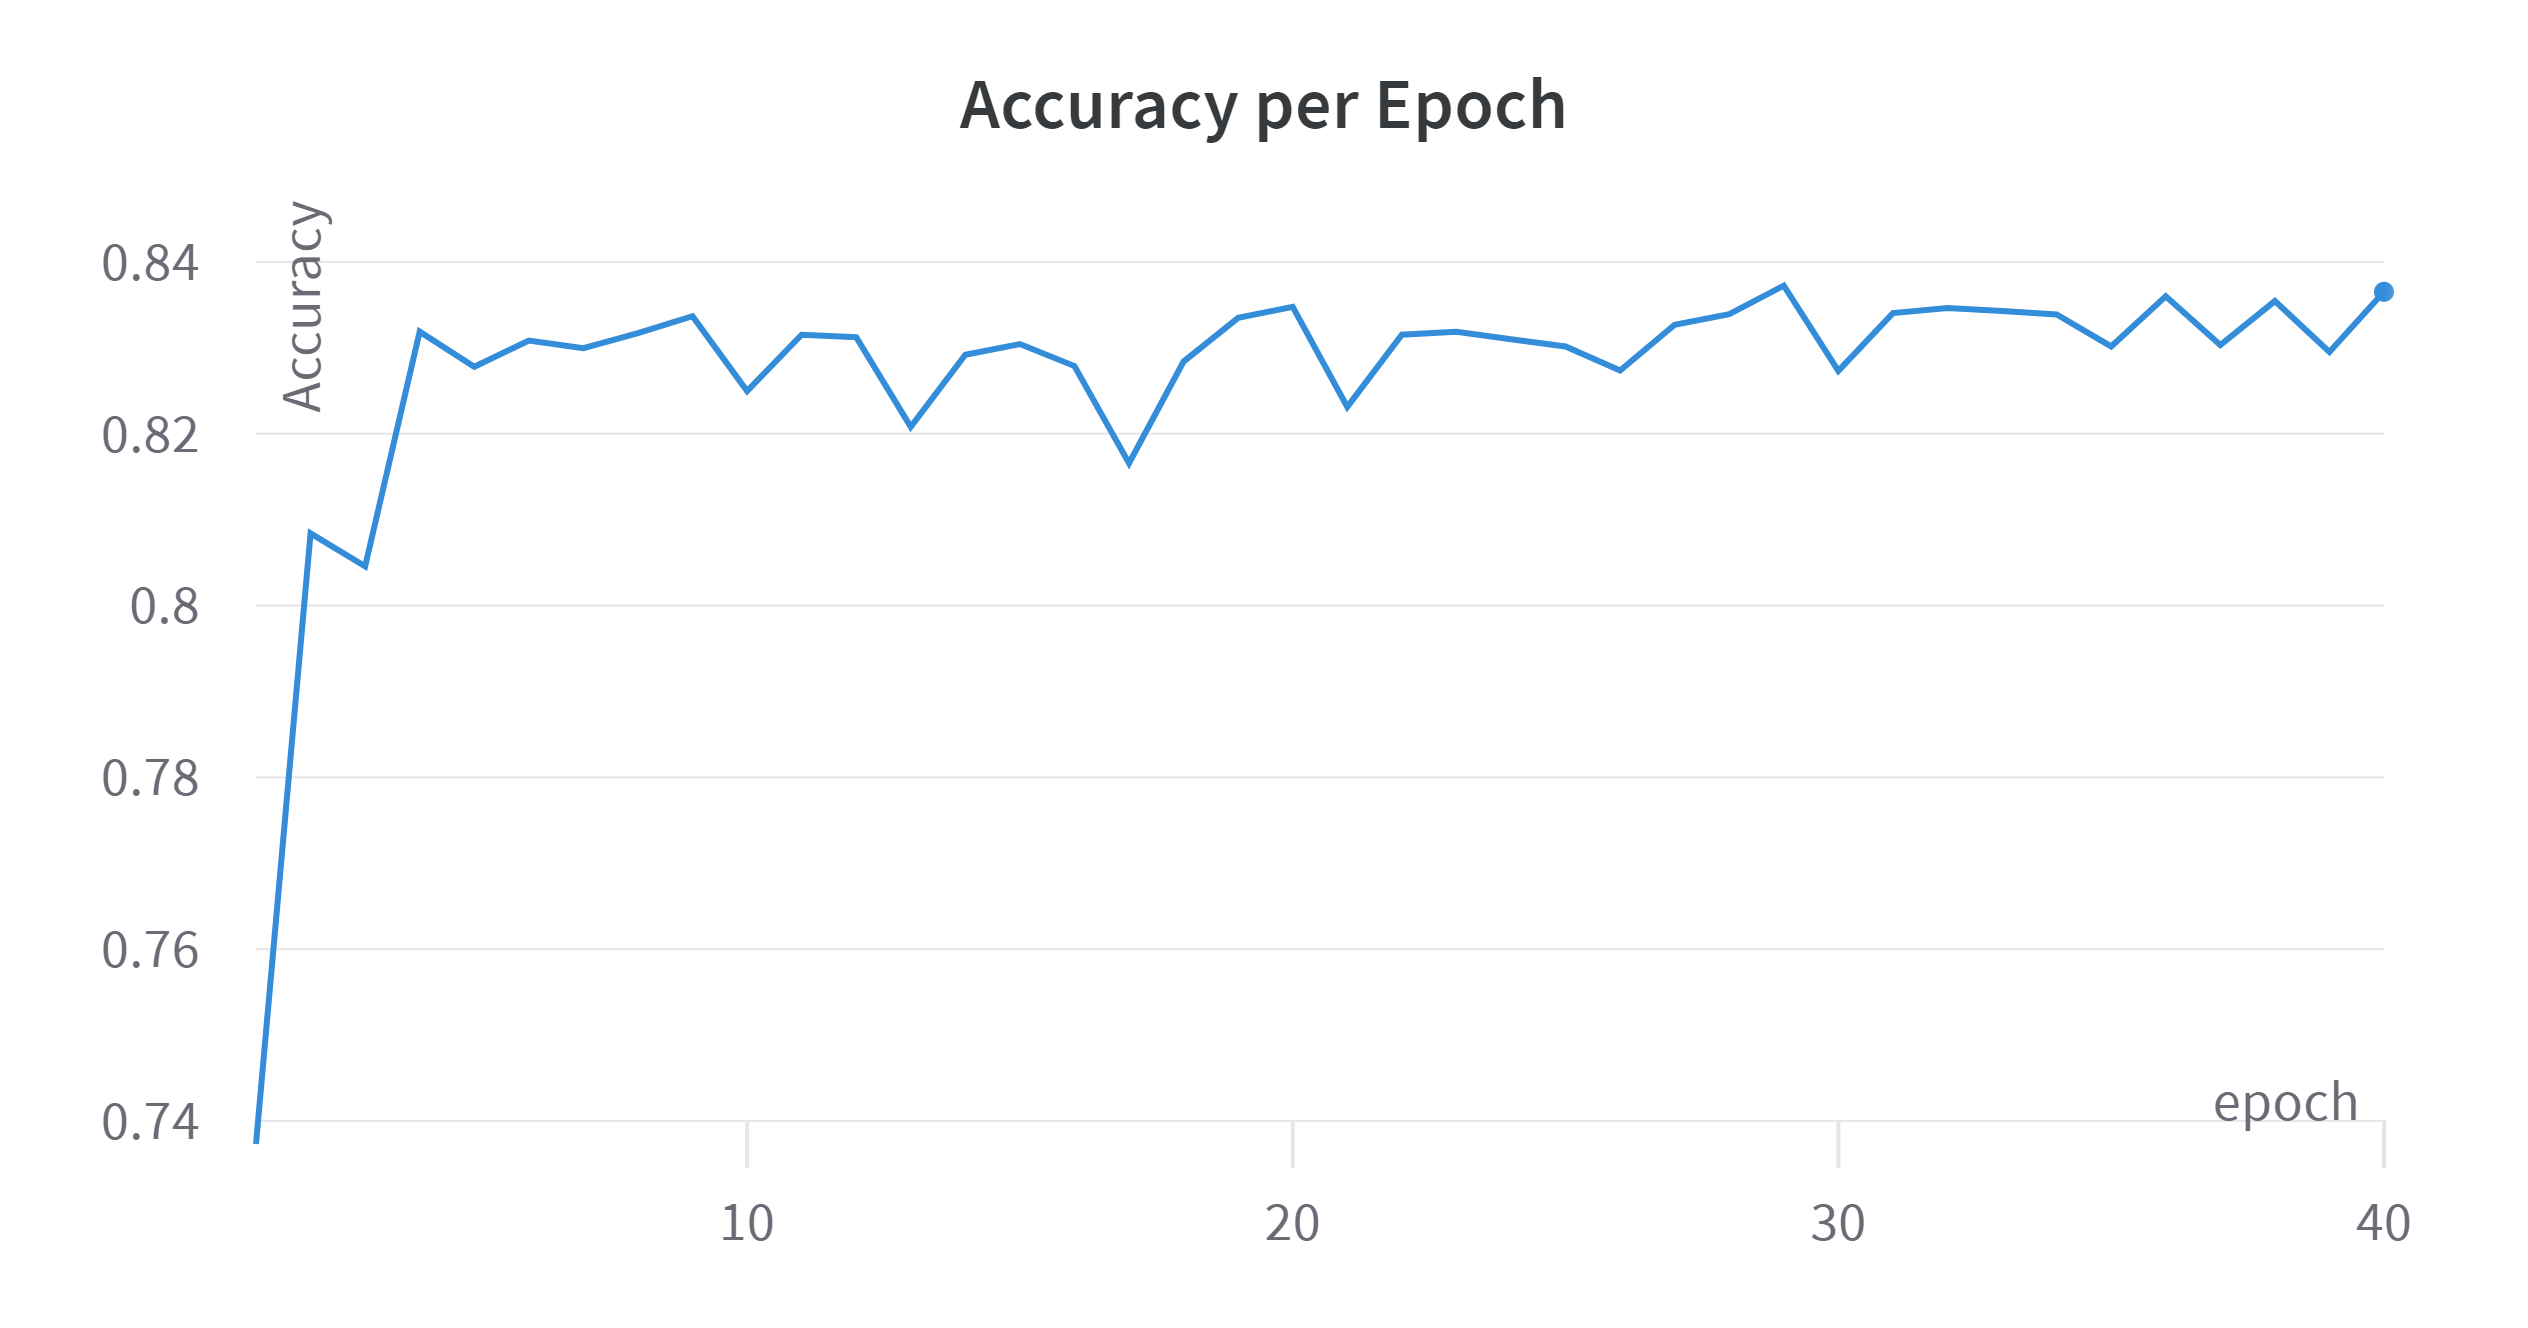
\includegraphics[scale=0.20]{q5/Accuracy-per-Epoch.png}
\subsection{}
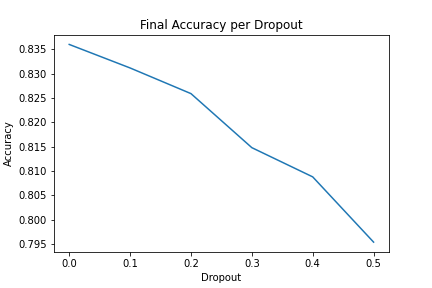
\includegraphics{q5/acc_per_dropout.png}
\subsection{}
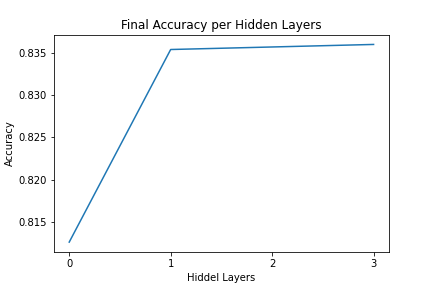
\includegraphics{q5/acc_per_hl.png}
\subsection{}
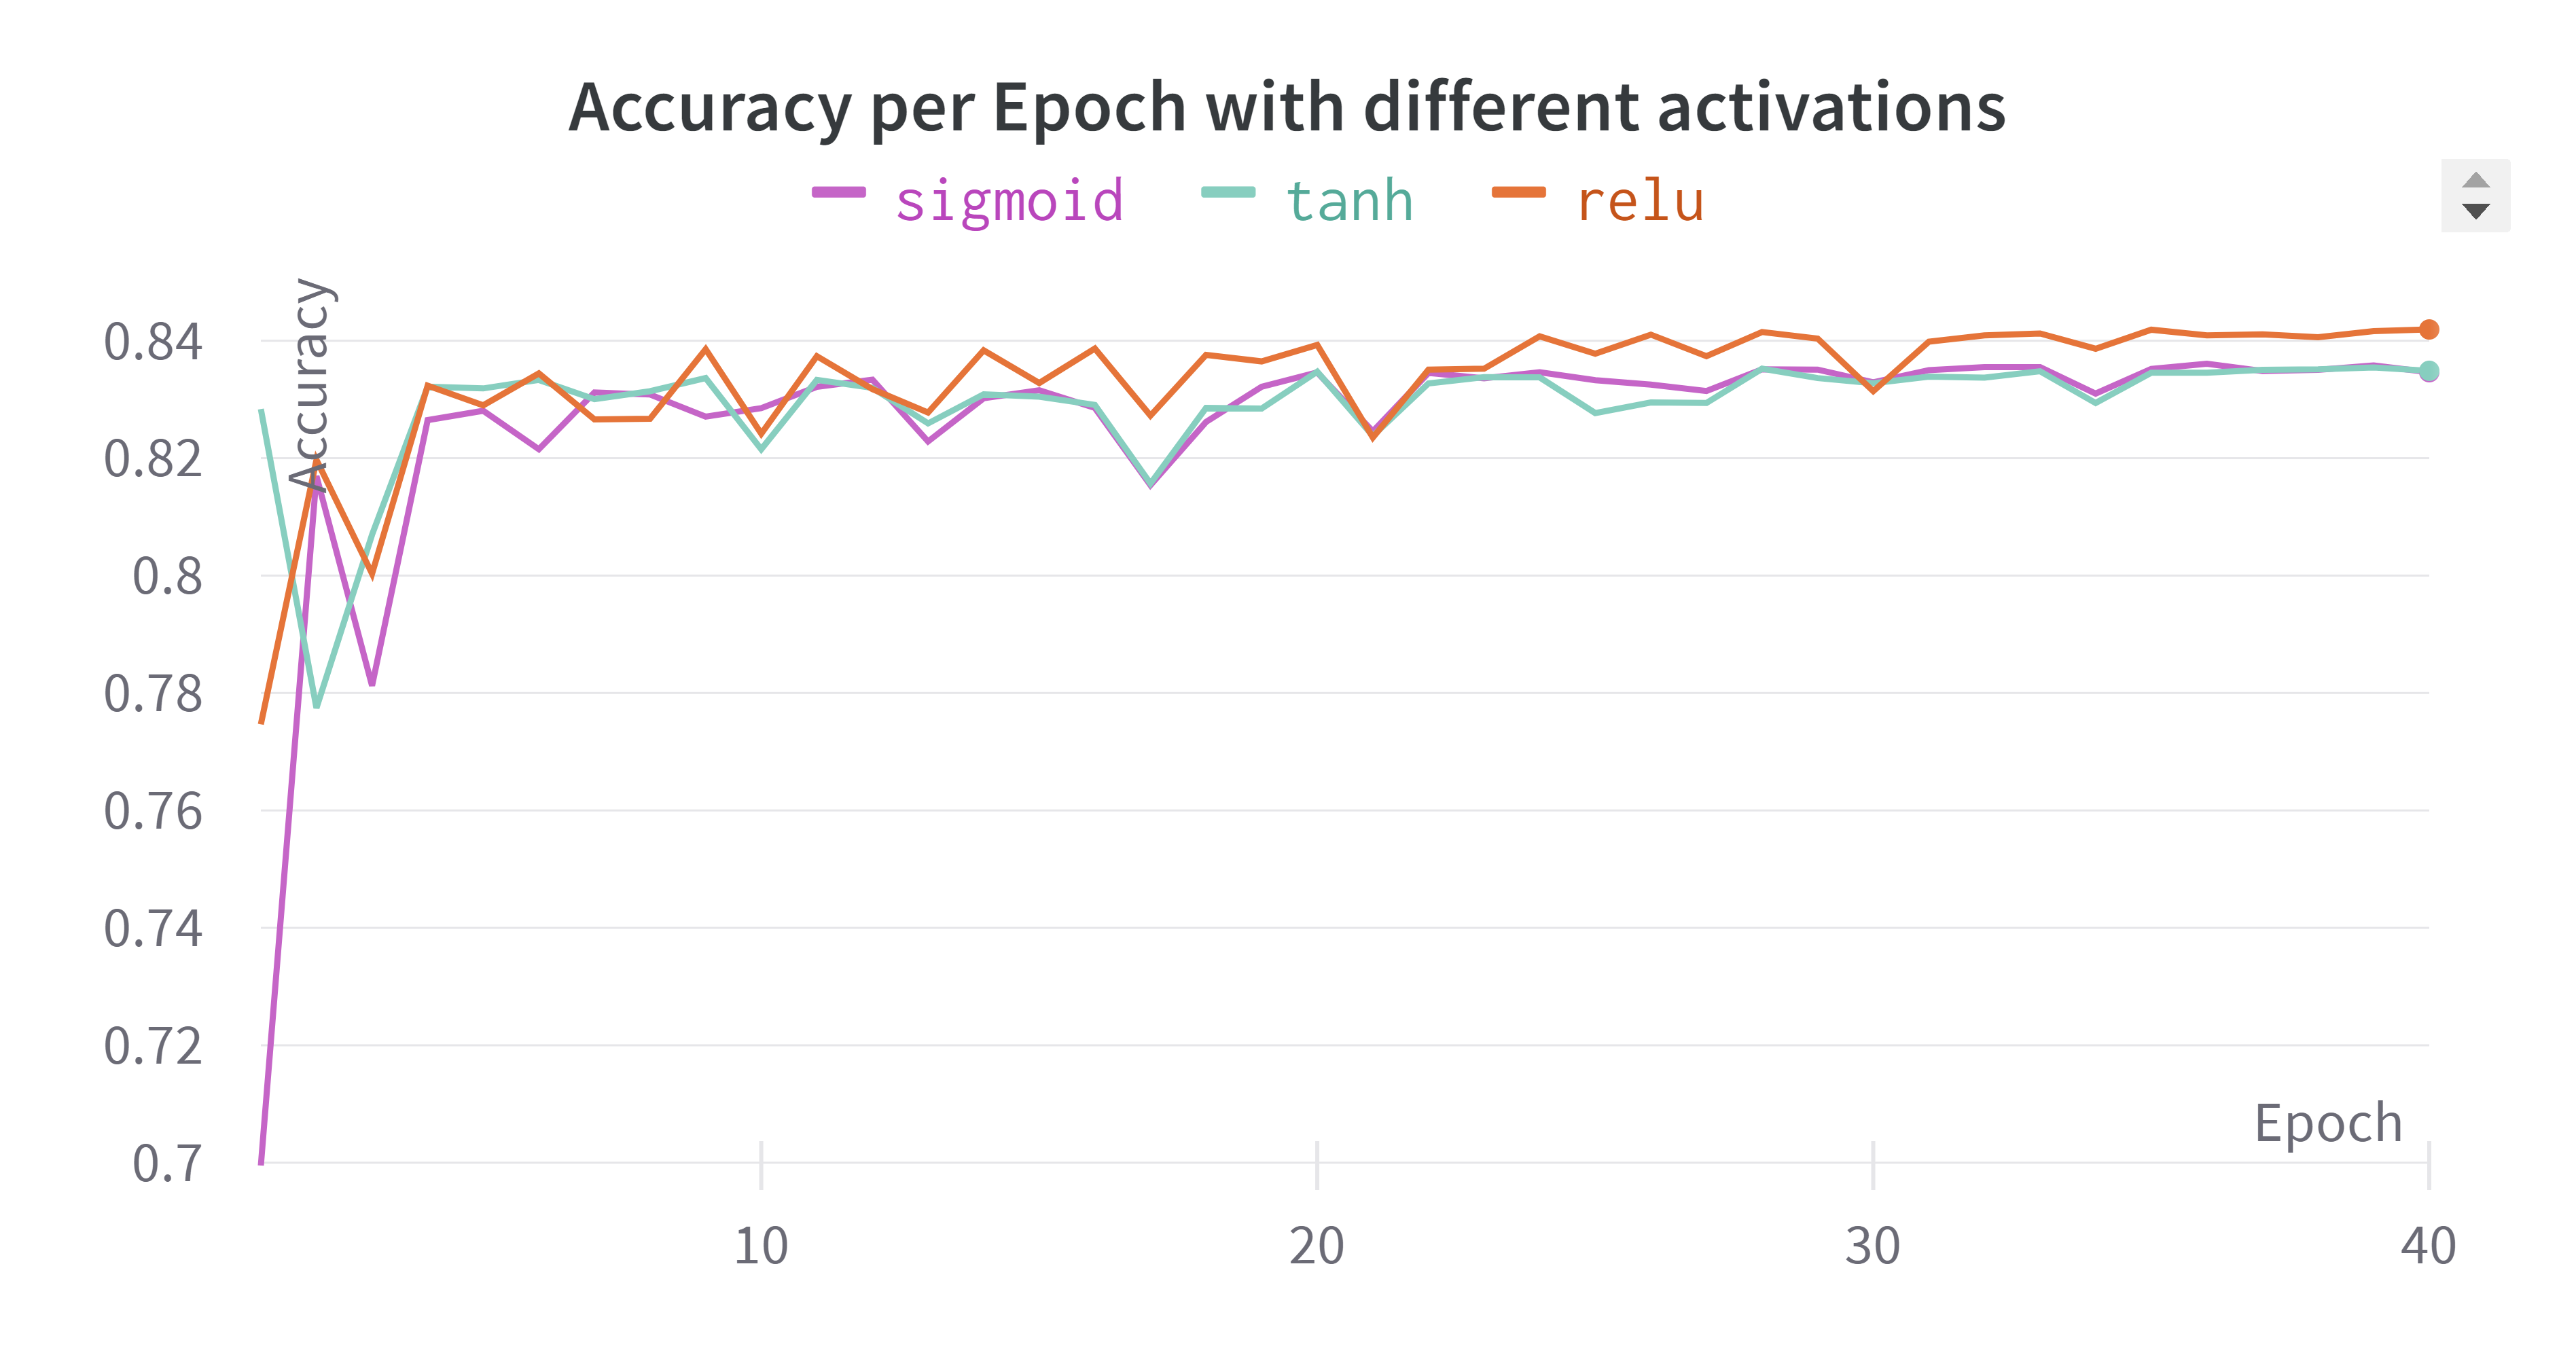
\includegraphics[scale=0.12]{q5/different_activations.png}
\subsection{}
\newenvironment{simplechar}{%
   \catcode`\$=12
   \catcode`\&=12
   \catcode`\#=12
   \catcode`\^=12
   \catcode`\_=12
   \catcode`\~=12
   \catcode`\%=12
   \catcode`\<=12
   \catcode`\>=12
}{}
\begin{simplechar}
Example 1:
This is the latest entry in the long series of films with the French agent, O.S.S. 117 (the French answer to James Bond). The series was launched in the early 1950's, and spawned at least eight films (none of which was ever released in the U.S.). 'O.S.S.117:Cairo,Nest Of Spies' is a breezy little comedy that should not...repeat NOT, be taken too seriously. Our protagonist finds himself in the middle of a spy chase in Egypt (with Morroco doing stand in for Egypt) to find out about a long lost friend. What follows is the standard James Bond/Inspector Cloussou kind of antics. Although our man is something of an overt xenophobe,sexist,homophobe, it's treated as pure farce (as I said, don't take it too seriously). Although there is a bit of rough language & cartoon violence, it's basically okay for older kids (ages 12 & up). As previously stated in the subject line, just sit back,pass the popcorn & just enjoy.

Example 2:
I was expecting "Born to Kill" to be an exciting, high-tension film noir. Instead, it's got two good action set-pieces (one at the beginning and one at the end) and some marvelously atmospheric cinematography by Robert de Grasse (usually a "glamor" cameraman and a surprising credit for a noir), but the rest of the film is pretty boring. Lawrence Tierney goes through his psycho kick but it's a strictly by-the-numbers performance, mechanically churning out what the audience expected from him after "Dillinger" (an overrated movie but at least better than this). Claire Trevor's character is too stupid and unmotivated to have any audience appeal, and the action (such as it is) stays so resolutely inside that damned house in San Francisco the film becomes claustrophobic instead of genuinely thrilling. It's one of those movies in which the supporting players -- notably Elisha Cook, Jr. (whose character's homoerotic itch for Tierney's is one of the few subtleties in an otherwise pretty obvious script) and Isabel Jewell -- out-act the leads. It also doesn't help that, nearly half a century after Alfred Hitchcock and Anthony Perkins revolutionized the depiction of psycho killers on the screen in "Psycho," Tierney's is so gross and obvious he might as well have "PSYCHO" tattooed on his forehead. Also, there's no indication in the film as it stands as to why the source novel was called "Deadlier than the Male" -- but perhaps James Gunn made the female characters stronger and more interesting than they are in the film. "Born to Kill" is a real disappointment from Robert Wise, who already had some quality movies under his belt and would go on to a stellar career.

Example 3:
It seems everyone wants to jump on the bandwagon and say "Maha Go Go Go"....The word is MACHA........Like "Mach".....Pronounced maa - ka"...<br /><br />I grew up with this series in the early 70's here in LA on the late and VERY lamented channel 56...Before that there was Tetsuwan Atomu (Astro Boy), dating from 1963 on ol' KHJ TV. Astro Boy was the first TV example of anime we got here in the states...I was into anime as a kid and followed it until the late 80's when, by then it'd become a series of badly animated "talking heads", a phenomenon which has only gotten worse. 'Nuff said.<br /><br />As for "Speed Racer", I really enjoyed the basics there, the POV shots, the cinematic aspects of live action skillfully adopted to animation...That was fairly typical of most Japanese anime back then...Graphics graphics graphics! Take note sometime how obviously the series was inspired by Stanley Kramer's film "Grand Prix" (1966), especially the redone American credits....<br /><br />Oh yeah, I have the original comics from which the series is based, so I know of which I speak.<br /><br />What were we doing animation-wise besides crap like Johnny Quest?.....Th' same ol' stuff we'd been doin' since the 20's....Ho-hum!<br /><br />I guess the real problem I had/have with the way anime was/is shown on American TV is the hatchet job done on the scripts, credits, etc to "sanitize" them for American audiences...I won't go into other programs as we're talking' Speed here.<br /><br />Look at clowns like Peter Fernandez as one of the culprits here, as he was 99% responsible for the re-writes of the series...Not to mention the voice of Speed, Racer X and others...Between him and the goofs at Trans/Lux ( Think Felix the Cat and the Mighty Hercules - oy vey!) they took a slick, very sophisticated show and dropped it down to the level of Sesame Street. Think "Cruncher Bloch", The "Forthebird Company", "Skull Duggery"...If I go on I'll puke.<br /><br />This series dates from 40-odd years ago but I, at the time, was keen enough to feel insulted by the dumbing down of this and other Japanese programs...I mean it's obvious when someone's getting' killed but they either remove it or gloss it over........Pleeeeeze!<br /><br />Good show - originally. Sadly all the more recent incarnations of the series have that CRAPPY "made in Korea" look, not to mention being nauseatingly "pc" in content. Even the Japanese outsource their animation now..<br /><br />Try watchin' the original Japanese opening on YouTube sometime...It sends chills up my spine.....If only......Oh well. Robert

Example 4:
Recap: Since the warrior queen Gedren raised and slaughtered most of Sonja's family, she has trained in the art of sword fighting. Now, Gedren has taken a very powerful talisman, that threatens to destroy the world if not destroyed, killing Sonja's sister in the process. Now Sonja is out for revenge, and to save the world. Along the way, she meets the very Conan-like (but not Conan, no!) Kalidor, the child-prince Tarn and his bodyguard Falcon. At first Sonja declines all help, but is later forced to accept it, and together they go to save the world.<br /><br />Comments: When you watch a movie like this, and you think that it is the story that the is the best element in this movie, the movie is in big trouble. Because 1) a movie like this should draw its strength upon good swordfights and effects, and 2) the story is really, really bad. It is simple, and uncomplicated and really offers nothing in way of character development or even suspense. It is predictable and boring, and the obvious couple, Sonja and Kalidor, has no chemistry at all. And the kid is just annoying. And most of the scenes is drawn out so long that they become boring. Though the movie is not very long, it has not material enough to fill its time. And so back to point 1). The fighting is slow, uneventful and really bad. It clearly shows most fighters clearly blocking the opponents strokes far ahead of the opponent has even begun to strike. In my honest opinion, I believe most kids, fighting with sticks, creates more exciting fights playing knights than this movie did. All in all, this is a really bad spin-off, that should be avoided by all who liked the Conan-movies.<br /><br />2/10

Example 5:
Not as bad as some people say...This is a unofficial Bond movie and a remake of "Thunderball", written by Kevin McClory (co- producer in "Thunderball"). Well, the cast is very very interesting, Maria Brandauer is a great Bond- villain, Kim Basinger and Barbara Carrera are just like the "original" Bond- girls, plus Rowan Atkinson and a truly great Edward Fox, who looks really refreshing in the "M" role. In fact, the whole movie is refreshing and gives some new impulses. Sean Connery does it once more confident and charming, except that he looks a little bit too old. But alright, he is the original Bond and it was great to see him once more in this role. The locations are also typical- Bahamas, France, etc. The only thing that really fails is the music score, the song "Never say never again" is O.K., but the theme song is just missing. All in one, a nice try to make a difference from the comic and silly Roger Moore movies like "Moonraker". Only if there was another story, "Thunderball" was a excellent movie and really did not needed a remake
\end{simplechar}


\section{Right-to-left vs left-to-right Estimation}
\subsection{}
Let's denote the left-to-right count-based bi-gram model as L and the right-to-left count-based bi-gram model as R. The probability estimates for each model are as follows:

$L(w | v) = \frac{C_{L}(w,v)}{C(v)}$ - Probability of $w$ given $v$ in the left-to-right model.

$R(w | v) = \frac{C_{R}(w,v)}{C(v)}$ - Probability of $w$ given $v$ in the right-to-left model.

Where $C_{L}(w,v)$ and $C_{R}(w,v)$ is counting the bi-gram sequence from left/right respectively.

Notice that by definition $C_{L}(w,v) = C_{R}(v,w)$

Also:

$L(x_i | x_{i-1}) = \frac{C_{L}(x_i,x_{i-1})}{C(x_{i-1})} = \frac{C_{R}(x_{i-1},x_i)}{C(x_{i-1})} = \frac{R(x_{i-1} | x_i)}{C(x_{i-1})}C(x_i)$

Estimating the bi-gram from left to right for a corpus of size $M$ gives:

$P(x_0x_1...x_n)=P(x_0)\Pi_{i=1,...,n}L(x_i | x_{i-1})=\frac{C(x_0)}{M}\prod_{i=1}^{n}L(x_i | x_{i-1})=
\frac{C(x_0)}{M}\prod_{i=1}^{n}\frac{R(x_{i-1} | x_i)}{C(x_{i-1})}C(x_i)$

Notice that we got a telescopic product which after cancelling elements equals:

$\frac{C(x_0)}{M}\frac{C(x_n)}{C(x_0)}\prod_{i=1}^{n}R(x_{i-1} | x_i) = \frac{C(x_n)}{M}\prod_{i=1}^{n}R(x_{i-1} | x_i)$

This is exactly estimating the bi-gram model with right to left count, which is what we wanted to prove.


\end{document}